\chapter{Background}
\label{ch:background}

This chapter presents the necessary background information for this thesis. First, we define some basic terminology that we use throughout this thesis. Next, we research prior work in the field of \acrshort{vr} that interfaces \acrshort{vtk} and Unity or develops \acrshort{ide}s for visualizations within a \acrshort{vr} environment. We also examine the software and solutions produced by these previous studies and extract which factors contribute to potential maintainability issues and which on the contrary make them more maintainable. 

\section{Terminology}

We define a set of terms that we use throughout this thesis. We use the \textit{Glossary of virtual reality terminology} \cite{manetta1995glossary} as a main source for our terminology.

\begin{itemize}[leftmargin=1.5truecm]
    \setlength{\itemindent}{-1truecm}
    \item[] \textbf{\acrfull{vr}} A computer system used to create an artificial world which is immersive and interactive for the user \cite{manetta1995glossary}.
    \item[] \textbf{Immersion} The feeling of the user of being part of a virtual environment \cite{manetta1995glossary}.
    \item[] \textbf{Virtual Environment} Realistic simulations of interactive scenes \cite{manetta1995glossary}.
    \item[] \textbf{Interactivity} The ability of the user to navigate and manipulate (objects in) the environment.
    \item[] \textbf{Visualization Toolkit} Library containing functionality aimed at creating and manipulating data visualizations.
    \item[] \textbf{Game Engine} A software that enables the creation of virtual environments.
\end{itemize}

\section{The Visualization Toolkit}

As the necessity to produce ever more complex visualizations grows, both in commercial and scientific settings, a number of visualization toolkits have been developed to support the development of these visualizations. These libraries tend to specialize on some form of visualization; for example, \acrfull{vtk} focuses on scientific visualization \cite{kruis_creating_2017} and \acrfull{itk} on image analysis \cite{yoo_engineering_2002}.

These toolkits come in a variety of flavours, languages and/or wrappings and it is thus out of the scope of this thesis to analyse and develop upon all of them. We will discuss research done on all three to create \acrshort{ide}s for or within \acrshort{vr} environments, but we will ultimately choose to use for a proof of concept. For this discussion, we will take into consideration the three aforementioned libraries.

\acrfull{vtk} is a library oriented towards \blockquote{manipulating and displaying scientific data}\footnote{\url{https://vtk.org/}}. It creates visualizations by means of filter pipelines, a technique proposed by Haber and McNabb \cite{haber1990visualization}. These filters manipulate input data through some set of transformations and return the composed data which can then be visualized. 

\acrshort{vtk} has three different stages of the pipeline which combined return a visualization rendering. The first stage is the generation or the import of a data source and transforming the raw data in some more readable raw data if needed, like structuring it in a model. Subsequently, the raw data is then transformed through filters that compose the data in order for it to be visualized, creating the actual visualization. Finally, the visualization is rendered through the application of mappers that transform the computational representation into a graphical representation. An example of a Quadric 3D function is shown in Figure~\ref{fig:quadric-render-pipeline}, based on an example proposed in the \acrshort{vtk} example repository\footnote{Available at \url{https://kitware.github.io/vtk-examples/site/Cxx/VisualizationAlgorithms/ContourQuadric/}.}, the exact code is presented in Appendix~\ref{apx:quadric-vtk}.

\begin{figure}
    \centering
    \begin{subfigure}{\textwidth}
        \centering
        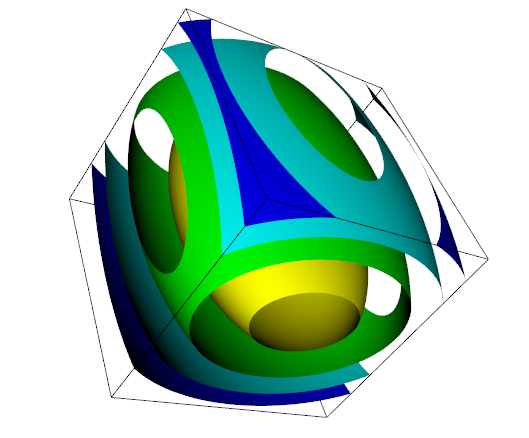
\includegraphics[width=0.7\textwidth]{pictures/Quadric-Rendering.PNG}
        \caption{}
    \end{subfigure}
    \begin{subfigure}{\textwidth}
        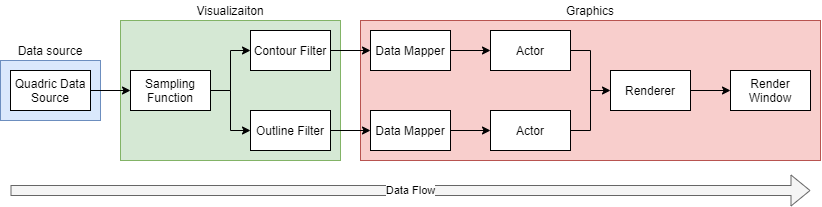
\includegraphics[width=\textwidth]{pictures/Pipeline-VTK-Quadric.png}
        \caption{}
    \end{subfigure}
    \caption{VTK visualization (a) and pipeline (b) of a sampled Quadric function.}
        \label{fig:quadric-render-pipeline}
\end{figure}

Upon \acrshort{vtk}, a number of wrappers have been produced, allowing the library to be used not only in C++, but also in Java, Python, Tcl and the .NET Framework\footnote{\url{https://vtk.org/Wiki/VTK/Wrappers}}. These wrappers allow the usage of the \textit{wrappable} code of the library from one of the aforementioned languages. This process is to be manually done at build time of the library or using one of the wrapping tools accessible from the documentation of \acrshort{vtk}.

\section{Game Engines}

Game Engines can be defined as \textit{software frameworks for game development} \cite{politowski2021game}. These frameworks though are not all equal, and as such we focus on those defined as \textit{\acrfull{gpge}s}, which we define as \textit{frameworks for the creation of virtual environments}, which is a fundamental component of games. This also means that these softwares are not restricted to game development purposes, but are used for a variety of projects that entail the simulation of virtual worlds. These frameworks perfectly fit our requirement of creating an immersive and interactive environment for our \acrshort{vr} IDE.

A number of \acrshort{gpge}s exist, such as Unity Engine \cite{haas2014history} and Unreal Engine \cite{unrealengine}. We will be using Unity as the engine on which we base our solution. This is ideal for our research as previous research already exists discussing the integration of \acrshort{vtk} and this engine \cite{wheeler_virtual_2018}. Furthermore, it is a very well established, used and supported engine.

We chose to use Unity due to the number of advantages that come with the engine. First and foremost, Unity has already a decent \acrshort{vr} integration with the OpenVR\footnote{\url{https://github.com/ValveSoftware/unity-xr-plugin}} and OpenXR\footnote{\url{https://docs.unity3d.com/Packages/com.unity.xr.openxr@0.1/manual/index.html}} plugins. The \acrshort{vr} community is already quite established and, in general, the development community is very active and offers valuable support. 

The documentation for the engine is comprehensive and freely available with a number of examples that facilitate development, and its API supports the implementation of custom native C++ code through easy drag-n-drop of the shared libraries in the editor and an intuitive interface to import its functionalities in C\#. Finally, thanks to OpenGL 2 context sharing, it is possible to render through external code, such as \acrshort{vtk}, which suites our need to visualize objects created in native C++ libraries.

\section{Related Work}

A number of projects already attempted interfacing visualization libraries with frameworks, be it \acrshort{gpge}s or IDEs, while others attempted the creation of visualization editors, albeit for different purposes and/or constraints. In this section we will discuss these previous attempts and how they contribute to laying the ground for our development.

\paragraph{OculusVTK Visual editor}

In 2016 a similar attempt to create a visual editor for OculusVTK was carried out in Python in a stand \cite{dreuning_visual_2016}. The solution allowed the user to create simple pipelines and manipulate them within a visual environment and see the result of the operations. The authors carry out a number of experiments with pipelines, varying from simple arrows to stream tracers and a DICOM image rendering, where results showed a consistent 58-60 FPS were achieved.

While the objectives of the authors are quite similar to ours, they do not focus on the same constraints we set for our project, i.e. performance and the designing of a distributable and parallelizable architecture. Furthermore, their solution focuses on Oculus, whereas our solution aims at being headset-agnostic.

The power of the solution proposed lays in its usage of Python's capability of introspecting on its modules and harvesting data in order to achieve a more general approach to interfacing with \acrshort{vtk}. We base our solution partly on this software, as we will discuss in Section~\ref{sec:design-introspection}.

\paragraph{VtkToUnity}

The closest attempt to our project was presented in 2018 by Wheeler et al. who developed a Native Unity plugin that allowed the user to exploit \acrshort{vtk}'s features in the engine's scripts\footnote{\url{https://gitlab.com/3dheart_public/vtktounity}}. The plugin's aim is to introduce volume rendering through \acrshort{vtk} and uses the OpenGL context sharing technology to enable the visualization library to directly render within the Unity scene. The plugin's approach is to add a rendering callback function after the transparency rendering stage, as optimal for volume rendering. The produced architecture is summarized in Figure~\ref{fig:wheeler-architecture} \cite{wheeler_virtual_2018}.

\begin{figure}
    \centering
    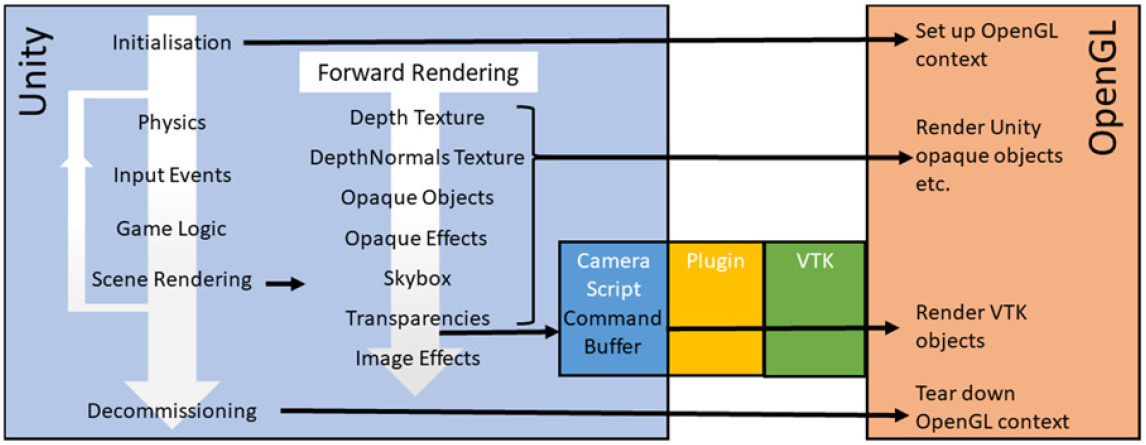
\includegraphics[width=\textwidth]{pictures/wheeler_arch.PNG}
    \caption{Wheeler et al.'s rendering architecture.}
    \label{fig:wheeler-architecture}
\end{figure}

The authors carry out experiments to evaluate the performances of the solution. Their objective frame rate is of 90 FPS using a HTC Vive \acrfull{hmd}, which aligns with Unity's own guidelines \cite{noauthor_vr_nodate-1} as well as the 90Hz refresh rate of the \acrshort{hmd} \cite{BuyVIVEH54}. With simpler renderings the solution is of its own able to achieve the desired frame rate, but with more complex scenes it does not. To overcome this, the authors propose the usage of setting the desired frame rate using \acrshort{vtk}'s own \verb|vtkExternalRenderingOpenGLRenderWindow::SetDesiredUpdateRate| to solve this.

This solution presents some limitations, as the C++ native code locks the shared API at every call, and as such limits the ability to leverage parallelization of the software, which could potentially aid the rendering quality while the objective frame rate is set. Furthermore, the plugin focuses on volume rendering in particular, while our solution aims at a more general solution. 

\paragraph{ActiViz}

Kitware, the company also maintaining \acrshort{vtk}, have created a wrapper for .NET of \acrshort{vtk}, ActiViz\footnote{\url{https://www.kitware.eu/activiz/}}. This wrapper is ready to be used with Unity, and exposes the same functionality of the library as other wrappers. This allows already for a good integration of the library and Unity.

The downside of this solution is its performance: as the wrapper requires CPU to GPU copies, with complex visualizations the performances drop significantly. This has already been discussed by Wheeler et al. \cite{wheeler_virtual_2018} and is one of the reasons that lead them to develop their own solution. 

\paragraph{ParaView}

Again developed by Kitware, Paraview\footnote{\url{https://www.paraview.org/}} is an \acrshort{ide} for the creation of visualizations mainly based on \acrshort{vtk}. This uses the same paradigm as \acrshort{vtk} for the creation of visualizations, that is by the means of pipelines. The software supports a \acrshort{vr} porting for the visualizations which feels clunky, as it is a rendering of 2D UIs in a 3D immersive and interactive environment, which hinders user experience.